\documentclass[%
autoref,
colorlinks,  
facsimile,   % отображать факсимиле диссертанта и ученого секретаря
]{disser}

\usepackage[%
  a4paper, mag=1000,
  left=2.5cm, right=1cm, top=2cm, bottom=2cm, headsep=0.7cm, footskip=1cm
]{geometry}

\usepackage{multicol}
\usepackage{listings}
\usepackage{cmap}
\usepackage{graphicx}
\usepackage{ifpdf}
\usepackage{xcolor}
\usepackage[colorlinks = true,%
            linkcolor = blue,%
            urlcolor  = blue,%
            citecolor = blue,%
            unicode = true, %
            anchorcolor = blue]{hyperref}
\usepackage{hypernat}
\usepackage{wrapfig}
\usepackage{subcaption}
\lstset{language=C} 

\usepackage{hyphenat}
\usepackage[intlimits,fleqn]{amsmath}
\usepackage{pifont}
\usepackage{multirow}
\usepackage{amssymb,amsfonts,amsthm}
\usepackage[T2A]{fontenc}
\usepackage[utf8]{inputenc}
\usepackage[autostyle]{csquotes}
\usepackage[english,russian]{babel}
\usepackage{tabularx}
\usepackage{tikz}
\usepackage{pgfplots}
\usepackage{setspace}
\ifpdf\usepackage{epstopdf}\fi

\linespread{1.3}

\usepackage[%
    style=gost-numeric,
    backend=biber,
    bibencoding=utf8,
    sorting=none,
    bibstyle=gost-numeric,
    citestyle=numeric-comp,
    language=auto,
    autolang=other,
    sortcites=true,
    maxbibnames=6,
    defernumbers=true,
    movenames=false,
    doi=false,
    isbn=false,
]{biblatex}

\DeclareSourcemap{
    \maps{
        \map[overwrite]{ % переделка формата записи даты
            \step[fieldsource=urldate,
            match=\regexp{([0-9]{2})\.([0-9]{2})\.([0-9]{4})},
            replace={$3-$2-$1$4}, % $4 вставлен исключительно ради нормальной работы программ подсветки синтаксиса, которые некорректно обрабатывают $ в таких конструкциях
            final]
        }
    }
}
\DeclareFieldFormat{url}{\url{#1}} % Убирает URL: 

\usepackage[intoc,nocfg,russian]{nomencl}
\newcommand{\nomencl}[2]{#1 --- #2\nomenclature{#1}{#2}}
\setlength{\nomlabelwidth}{3em}
\setlength{\nomitemsep}{-\parsep}
\renewcommand{\nomlabel}[1]{#1 ---}
\makenomenclature

\renewcommand*{\newblockpunct}{%
    \addperiod\space\bibsentence}%block punct.,\bibsentence is for vol,etc.
\renewcommand*{\mkgostheading}[1]{#1} % только лишь убираем курсив с авторов

\addbibresource{references_autoref.bib}
\defbibheading{authorcited}{\nsection{Публикации автора по теме диссертации}}
\defbibheading{cited}{\nsection{Цитированная литература}}

\newtheorem{theorem}{Теорема}{\bfseries}{\itshape}
\newtheorem{statement}{Утверждение}{\itshape}{\rmfamily}
\newtheorem{lemma}{Лемма}{\bfseries}{\itshape}

\usepackage{wrapfig}

\addbibresource{references.bib}
\defbibheading{authorcited}{\nsection{Публикации автора по теме диссертации}}

\AtNextCitekey{\!}

% Номера страниц снизу и по центру
\pagestyle{footcenter}
\chapterpagestyle{footcenter}

% Путь к файлам с иллюстрациями
\graphicspath{{fig/}}

\newcommand{\IntroCite}{\Cite}
\DeclareCiteCommand{\Cite}{}{}{}{}

\begin{document}
% Включение файла с общим текстом диссертации и автореферата
% (текст титульного листа и характеристика работы).
% Общие поля титульного листа диссертации и автореферата
\institution{Федеральное государственное бюджетное учреждение науки \\ Институт системного программирования им. В.П.~Иванникова \\ Российской академии наук (ИСП РАН)}

\topic{Методы декомпозиции систем и моделирования окружения программных модулей для верификации Си-программ}
\author{Захаров Илья Сергеевич}

\specnum{05.13.11}
\spec{математическое и программное обеспечение\\ 
вычислительных машин, комплексов и компьютерных сетей}

\sa{Петренко Александр Константинович}
\sastatus{д.~ф.-м.~н., проф.}

\city{Москва}
\date{\number\year}

\mkcommonsect{objective}{Цели и задачи работы.}{%

{\bf Цель работы} --- развитие методов верификации крупных программных систем на языке программирования Си с использованием инструментов верификации моделей программ при помощи автоматизации декомпозиции системы на модули и синтеза моделей их окружения для сокращения трудоемкости и сроков верификации.

Для достижения поставленной цели были решены следующие задачи:
\begin{enumerate}
    \item Исследовать существующие подходы к применению инструментов верификации моделей программ для проверки требований к Си-программам и выявить проблемы, препятствующие расширению применения этих подходов на практике.
    \item Разработать архитектуру системы верификации Си-программ, выполняющей генерацию и решение набора верификационных задач при помощи автоматизированной декомпозиции системы на модули и синтеза моделей окружения модулей.
    \item Разработать метод автоматизированной декомпозиции Си-программ на модули.
    \item Разработать метод автоматизированного синтеза моделей окружения модулей, позволяющий адаптировать процесс синтеза для проверки разных видов требований и программ.
    \item Реализовать систему верификации моделей Си-программ на основе разработанных архитектуры и методов, оценить реализацию системы верификации на практике.
\end{enumerate}
}

\mkcommonsect{novelty}{Научная новизна.}{%

Научной новизной обладают следующие результаты работы:
\begin{itemize}
\item Метод автоматизированной декомпозиции Си-программ на модули.
\item Метод спецификации моделей окружения модулей Си-программ на основе композиции систем переходов и доказательство теоремы об изоморфизме множеств достижимых ошибочных состояний спецификации и результата ее трансляции на язык Си.
\item Метод автоматизированного синтеза моделей окружения модулей, позволяющий адаптировать процесс синтеза для проверки разных видов требований и программ.
\end{itemize}
}

\mkcommonsect{method}{Методология и методы исследования.}{%

Результаты диссертации были получены с использованием методов и моделей, применяемых при проведении верификации моделей программ. Математическую основу данной работы составляют теория графов, теория множеств, математическая логика и системы переходов.
}


\mkcommonsect{results}{Положения, выносимые на защиту.}{%

\begin{itemize}
    \item Метод автоматизированной декомпозиции Си-программ на модули.
    \item Метод спецификации моделей окружения модулей на основе композиции систем переходов.
    \item Метод автоматизированного синтеза моделей окружения модулей, позволяющий адаптировать процесс синтеза для проверки разных видов требований и программ.
\end{itemize}

На основе предлагаемых методов была реализована система верификации Klever, предназначенная для проверки требований к программным системам на языке программирования Си с расширениями GNU методом верификации моделей программ. Продемонстрировано, что разработанная архитектура системы верификации позволяет проводить верификацию на различных многоядерных и распределенных вычислительных системах.

}

\mkcommonsect{aprob}{Степень достоверности и апробация результатов.}{%

Основные результаты работы обсуждались на конференциях:
\begin{itemize}
\item 55-я научная конференция МФТИ (г.~Москва, 2012 год).
\item Международная научная конференция студентов, аспирантов и молодых учёных «Ломоносов-2013» (г.~Москва, 2013 год).
\item 7-й весенний/летний коллоквиум молодых исследователей в области
программной инженерии (SYRCoSE, г.~Казань, 2013 год).
\item 10-я конференция разработчиков свободных программ (OSSDEVCONF, г.~Калуга, 2013 год).
\item Международная Ершовская конференция по информатике\linebreak (PSI:~Perspectives of System informatics, г.~ Санкт-Петербург, 2014 год).
\item 5-й международный семинар Linux Driver Verification (г.~Москва, 2015 год).
\item 10-я летняя школа Microsoft Research (г.~Кембридж, Великобритания,
2015 год).
\item 1-й международный семинар, посвященный инструменту CPAchecker \\(г.~Пассау, Германия, 2016 год).
\item 2-й международный семинар, посвященный инструменту CPAchecker \\(г.~Падерборн, Германия, 2017 год).
\item 5-я Международная научно-практическая конференция «Инструменты и методы анализа программ» (г.~Москва, 2017 год).
\item Международная Ершовская конференция по информатике\linebreak (PSI:~Perspectives of System informatics, г.~Москва, 2017 год).
\item 5-я научно-практическая конференция OS DAY (г.~Москва, 2018 год).
\item Научно-практическая открытая конференция ИСП РАН им. В.П.~Иванникова (г.~Москва, 2018 год).
\item Семинар ИСП РАН (г.~Москва, 2018 год).
\end{itemize}
}

\mkcommonsect{pub}{Публикации и зарегистрированные программы.}{%

% Публикации
По теме исследования опубликовано 11 работ \parencite{Syrcose,EnvTrudy,configurable:Trudy,Zakharov2015,ZakharovEnv2015,ZakharovEnvPsi,subsystems:Trudy,survey:new,klever:new,Novikov:2018:ISOLA,Zakharov:2018:ISPRAS} из них 9 в изданиях перечня ВАК~\cite{EnvTrudy,configurable:Trudy,Zakharov2015,ZakharovEnv2015,ZakharovEnvPsi,subsystems:Trudy,survey:new,klever:new,Novikov:2018:ISOLA} и 6 входят в международную систему цитирования Scopus~\cite{Zakharov2015,ZakharovEnv2015,ZakharovEnvPsi,survey:new,klever:new,Novikov:2018:ISOLA}.
В совместных работах~\cite{configurable:Trudy,Zakharov2015} личный вклад автора заключается в описании метода моделирования окружения, а в работах ~\cite{EnvTrudy,ZakharovEnv2015,ZakharovEnvPsi} в описании реализации метода моделирования окружения в системе верификации LDV~Tools.
В совместных работах~\cite{subsystems:Trudy,klever:new,Novikov:2018:ISOLA} личный вклад автора состоит в описании методов декомпозиции программ на модули, а также спецификации и синтеза моделей окружения.

% Патенты
В ходе выполнения работы было получено 4 свидетельства о государственной регистрации программ для ЭВМ:
\begin{enumerate}
\item Свидетельство о государственной регистрации программы для ЭВМ \\№~2015662948: «Программный компонент решения задач верификации посредством использования инфраструктуры облачного сервиса».
\item Свидетельство о государственной регистрации программы для ЭВМ \\{№~2017660773}: «Klever Linux Kernel Verification Objects Generator».
\item Свидетельство о государственной регистрации программы для ЭВМ \\№~2017660774: «Klever Environment Model Generator for Linux Kernel\linebreak Modules».
\item Свидетельство о государственной регистрации программы для ЭВМ \\№~2017660776: «Klever Verification Scheduler».
\end{enumerate}
}

\mkcommonsect{contrib}{Личный вклад автора.}{%

Все представленные в диссертации результаты получены лично автором.
\pagebreak
}

\mkcommonsect{struct}{Структура и объем диссертации.}{%

Диссертация состоит из введения, обзора литературы, 5 глав, заключения и библиографии.
Общий объем диссертации 157 страниц, включая 10 рисунков и 14 таблиц.
Библиография включает 143 наименования на 18 страницах.
}


\title{АВТОРЕФЕРАТ\\
диссертации на соискание ученой степени\\
кандидата физико-математических наук}

\maketitle

% Внутренняя сторона обложки
\thispagestyle{empty}
%\vspace*{-2cm}
\noindent

\begin{singlespace}
Работа выполнена в Федеральном государственном бюджетном учреждении науки <<Институт системного программирования им. В.П.~Иванникова Российской академии наук>>.
\end{singlespace}

\vskip1ex
\begin{singlespace}
\noindent
\begin{tabularx}{\linewidth}{@{}lX@{}}
  \textbf{Научный руководитель:} & \textbf{Петренко Александр Константинович} \\
  & доктор~физико-математических~наук, \break профессор \\
  \textbf{Официальные оппоненты:} 
  & \textbf{Тормасов Александр Геннадьевич}\\
  & доктор~физико-математических~наук, профессор, ректор автономной некоммерческая организации высшего образования <<Университет Иннополис>> \\
  & \textbf{Буренков Владимир Сергеевич}\\
  & кандидат~технических~наук, разработчик-исследователь акционерного общества <<Лаборатория Касперского>> \\
  \textbf{Ведущая организация:} & Федеральное государственное учреждение \\
  & <<Федеральный исследовательский центр Институт прикладной математики \break им.~М.В.~Келдыша Российской академии наук>>
\end{tabularx}
\end{singlespace}

\vskip2ex\noindent
\begin{singlespace} 
Защита состоится <<23>> мая 2019 года в 15:00 на заседании диссертационного совета Д 002.087.01 при Федеральном государственном бюджетном учреждении науки «Институт системного программирования им. В.П.~Иванникова Российской академии наук», расположенном по адресу:
109004, Москва, ул. Александра Солженицына, 25.
\end{singlespace} 

\vskip1ex\noindent

\begin{singlespace} 
С диссертацией можно ознакомиться в библиотеке и на сайте
Федерального государственного бюджетного учреждения науки «Институт системного программирования им. В.П.~Иванникова Российской академии наук».
\end{singlespace} 

\vskip1ex\noindent
Автореферат разослан \datefield{}

\vskip2ex\noindent

\vfill\noindent
\begin{minipage}[b]{0.5\linewidth}
  Ученый секретарь\\
  диссертационного~совета~Д.002.087.01,\\
  кандидат физико-математических наук%, \emph{ученое звание}
\end{minipage}
\hfill
% вставка файла, содержащего факсимиле ученого секретаря
\makeatletter
\ifDis@facsimile
  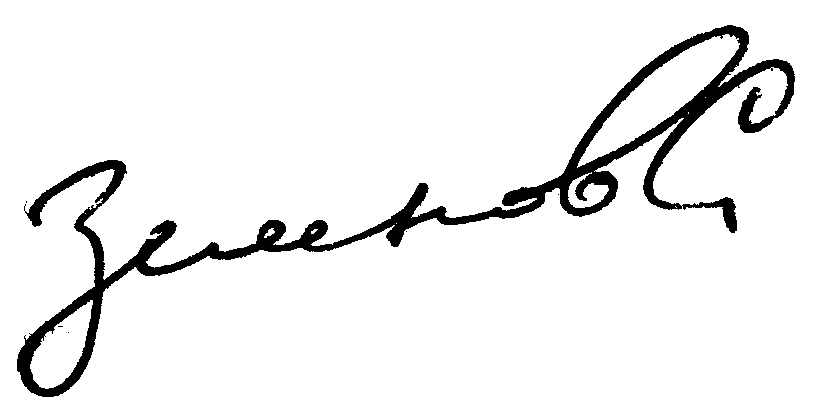
\includegraphics[width=3cm]{sec-facsimile}\hfill
\fi%
\makeatother%
Зеленов С.В.

\clearpage

\nsection{Общая характеристика работы}

% Общие разделы автореферата и диссертации
\mkcommonsect{actuality}{Актуальность темы исследования.}{%

Вопросам надежности и информационной безопасности в современном мире уделяется все больше внимания.
Одним из условий обеспечения надежности и защищенности операционных систем, систем управления базами данных, веб-серверов и других крупных программ на языке программирования Си, размер которых может достигать сотен тысяч и миллионов строк кода, является их верификация на разных этапах жизненного цикла.
Особенно остро стоит задача верификации крупных программных систем ответственного назначения, используемых в органах государственной власти, транспортной, космической, авиационной и других отраслях.

Подходы, основанные на формальных методах верификации программ, до последнего времени из-за низкой масштабируемости применялись либо к моделям, разрабатываемым на языках формальной спецификации, либо к небольшим программам.
На сегодняшний день уровень развития методов и инструментов уже позволяет выполнять проверку отдельных модулей программных систем на языке программирования Си. 
Работы по внедрению таких методов в промышленность особенно в отраслях, связанных с созданием программных систем ответственного назначения, постепенно выходят из фазы экспериментов и уже включаются в требования международных стандартов, например, ISO/IEC 15408 (Common Criteria), ISO/IEC 15408-1:2009, а также отраслевых стандартов в сфере транспорта ISO 26262-6:2018, EN50128, IEC 62279:2015 и авионики DO-178C.
Для последнего из упомянутых стандартов было разработано отдельное приложение DO-333, посвященное применению формальных методов.

Одним из направлений верификации программ на основе формальных методов является проверка требований к модулям программной системы при помощи метода верификации моделей (англ. software model checking).
Данный подход заключается в автоматическом построении модели программы на основе ее исходного кода, а затем ее формальной верификации на соответствие некоторому требованию.
Главным достоинством такого подхода на практике является возможность обнаруживать ошибки, которые существенно снижают надежность и информационную безопасность всей системы в целом и которые в рассматриваемых модулях трудно выявить при помощи других подходов к верификации программ.
К таким ошибкам относятся, например, некорректная работа с памятью, переполнение целочисленного типа, гонки по данным в параллельных программах, некорректное использование определенного программного интерфейса.

Активное развитие методы верификации моделей программ получили благодаря работам Рупака Маджумдара и Дирка Бейера, авторам одного из первых инструментов верификации Си-программ BLAST; исследователей компании Майкрософт, разработавших и внедривших серию инструментов SLAM, SLAM2, Yogi и Q; исследовательской группе Оксфордского университета, развивающей проект CBMC под руководством Даниеля Кроенинга.
Высокая трудоемкость работы инструментов верификации моделей программ все еще не позволяют применять данный подход к программным системам, размер которых приближается и даже превышает миллионы строк на языке программирования Си.
Для автоматизированного применения инструментов были построены системы верификации SDV, LDV~Tools и DC2, но реализованные в них методы применимы только к специализированным программам таким, как драйверы и программное обеспечение встраиваемых систем.
Поэтому развитие данного метода верификации крупных программных комплексов является актуальным.

Для преодоления ограничений существующих в настоящее время систем верификации моделей Си-программ в случае, когда размеры проверяемой программной системы достигают нескольких сотен тысяч или миллионов строк кода, в данной работе предлагается следующее: перед верификацией провести декомпозицию системы на модули, учитывая ограничения как самих инструментов верификации; затем обеспечить условия применимости инструментов верификации, а именно: подготовить модели окружения модулей, поскольку инструмент верификации принимает на вход структурно полную программу на языке Си; далее, для того чтобы время верификации было приемлемым на практике, нужно использовать средства распараллеливания процесса верификации, которые доступны на современных многоядерных и распределенных вычислительных системах. 
В совокупности развитие методов и систем верификации в перечисленных направлениях позволит сократить трудоемкость и время верификации программ.
}

\mkcommonsect{value}{Теоретическая и практическая значимость.}{%

Предложенные в диссертации методы реализованы в системе верификации Klever для проверки требований к программным системам на языке программирования Си с расширениями GNU при помощи инструментов верификации моделей программ, разрабатываемой в Институте системного программирования им. В.П.~Иванникова РАН. 
Klever используется при проверке требований к модулям ядра операционной системы Linux, в которых при помощи данной системы верификации было найдено более ста ошибок.
Система верификации используется для поиска дефектов и уязвимостей по безопасности, а также может применяться для проведения сертификационных исследований.
Изложенные в данной работе результаты применяются в образовательном процессе на факультете ВМК МГУ и будут полезны для развития методов верификации моделей программных систем.
}

%
% Используемые далее команды определяются в файле common.tex.
%

% Актуальность работы
\actualitysection
\actualitytext

% Цели и задачи диссертационной работы
\objectivesection
\objectivetext

% Научная новизна
\noveltysection
\noveltytext

% Теоретическая и практическая значимость
\valuesection
\valuetext

% Методология и методы исследования
\methodsection
\methodtext

% Положения, выносимые на защиту
\resultssection
\resultstext

% Степень достоверности и апробация результатов
\aprobsection
\aprobtext

% Публикации
\pubsection
\pubtext

% Личный вклад автора
\contribsection
\contribtext

% Структура и объем диссертации
\structsection
\structtext

\nsection{Содержание работы}

\textbf{Во введении} обоснована актуальность диссертационной работы, сформулирована цель и аргументирована научная новизна исследований, показана практическая значимость полученных результатов.

В \textbf{первой главе} приведен обзор работ в области проверки требований к Си-программам при помощи метода верификации моделей.

Рассматривается подход проверки требований к модулям Си-программ.
Данный подход реализован в таких инструментах верификации моделей программ, как CPAchecker, CBMC, SLAM2, Yogi.
В 2012 году было организовано сообщество разработчиков инструментов верификации моделей программ SV"~COMP, которое на сегодня насчитывает порядка тридцати групп исследователей и инженеров. 
Данным сообществом были предложены единые форматы входных и выходных данных и вспомогательные средства для использования различных инструментов верификации моделей на практике.

Инструменты верификации моделей Си-программ принимают на вход \textit{верификационные задачи}.
Верификационная задача содержит препроцессированный исходный код некоторого модуля программы, размер которого не превышает нескольких десятков тысяч строк кода на языке программирования Си, спецификацию свойства корректности, конфигурационные параметры и ограничения на вычислительные ресурсы.
Инструменты верификации поддерживают небольшой набор свойств корректности таких, как, например, корректность работы с памятью, недостижимость ошибочного оператора, завершимость программы.
На практике задачу проверки определенного требования к программе сводят к проверке одного или нескольких поддерживаемых свойств корректности за счет разработки модели требования на языке программирования Си, которая добавляется к исходному коду верификационной задачи.
Результат решения верификационной задачи состоит из вердикта и свидетельства корректности или нарушения.
Вердикт может принимать значения \textbf{True}, если программа корректна, \textbf{False} при обнаружении нарушения свойства корректности или \textbf{Unknown}, например, если для верификации не хватило вычислительных ресурсов.
Свидетельства корректности или нарушения предназначены для экспертизы пользователем или автоматической валидации.
Схема работы инструментов верификации моделей программ изображена на рисунке~\ref{figure:vt}.

Для выполнения верификации крупной программной системы требуется декомпозировать исходный код на модули размером не более нескольких десятков тысяч строк на языке программирования Си и формализовывать требования.
Чтобы достичь результатов с низким числом пропущенных ошибок и ложных предупреждений об ошибках, для каждого модуля программы следует подготовить модель его окружения.
Модель окружения дополняет модуль до структурно-полной программы с единственной точкой входа (main), а также содержит модели релевантных проверяемому требованию неопределенных функций, вызываемых в модуле. 
Анализ данных работ показал, что главным ограничением при применении инструментов верификации моделей программ является высокая трудоемкость подготовки верификационных задач.

Далее рассматриваются подходы автоматизации применения инструментов верификации моделей программ к драйверам операционных систем (ОС) и встраиваемому программному обеспечению.
Данные подходы реализованы в системах верификации Microsoft SDV, LDV~Tools и DC2, которые показали возможность как получения результатов с высокой точностью, так и существенного снижения необходимых трудозатрат при верификации.
Системы автоматизируют подготовку верификационных задач, включая самые трудоемкие этапы: декомпозицию программ на модули, синтез моделей окружения и требований.

\begin{figure}
\centering
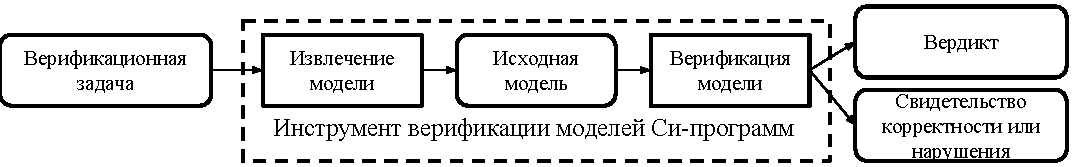
\includegraphics[scale=0.9]{vt}
\caption{Схема решения верификационных задач.}
\label{figure:vt}
\end{figure}

\begin{table}
\centering
\begin{tabular}{ | l | c | c | c | }
\hline
Критерий сравнения & SDV & LDV & DC2 \\
\hline
\begin{tabular}{@{}l@{}} Поддержка адаптивной декомпозиции программ\end{tabular} & \ding{55} & \ding{55} & \ding{55} \\
\hline
\begin{tabular}{@{}l@{}} Наличие средств для разработки или \\ исправления моделей окружения  \end{tabular} & \ding{51} & \ding{55} & \ding{55} \\
\hline
\begin{tabular}{@{}l@{}} Синтез моделей окружения\end{tabular} & \ding{55} & \ding{51} & \ding{51} \\
\hline
\begin{tabular}{@{}l@{}} Параллельные генерация и решение \\ верификационных задач\end{tabular} & \ding{55} & \ding{55} & \ding{55} \\
\hline
\end{tabular}
\caption{Сравнение систем верификации моделей программ.}
\label{table:systems}
\end{table}

В таблице~\ref{table:systems} представлен результат сравнительного анализа существующих систем верификации.
В системе верификации DC2 декомпозиция не выполняется, а SDV и LDV позволяют выделять в качестве модулей только драйверы без возможности корректировки состава модулей.
Разработчики системы верификации SDV подготовили модели окружения драйверов определенных видов на языке Си вручную без использования методов автоматизации.
Подход к автоматической генерации моделей окружения, реализованный в системе верификации LDV Tools, опирается на эвристические предположения и не позволяет повысить точность моделей окружения, что приводит к увеличению числа ложных предупреждений об ошибках.
Метод генерации моделей окружения, реализованный в системе верификации DC2, предназначен только для замены определений функций программы на упрощенные аннотации, что не позволяет описать вызов точек входа в таких моделях окружения.
Важным ограничением систем верификации является отсутствие средств для распараллеливания генерации и решения верификационных задач, из-за чего время верификации может превышать часы и даже дни.

Затем описываются работы в области распараллеливания алгоритмов верификации моделей.
Для верификации моделей Си-программ в данной работе отдается предпочтение методам параллельного решения верификационных задач с использованием вычислительных кластеров, построенных на основе IaaS (англ. Infrastructure as a Service) платформ и специализированных облачных сервисов.

В конце главы формулируется ряд основных требований к системам верификации моделей Си-программ, которые должны автоматизировать процесс генерации и решения верификационных задач.
Декомпозицию и синтез моделей окружения следует автоматизировать таким образом, чтобы пользователь имел возможность выполнять адаптацию данных процессов для проверки разных требований и программ.
Адаптацию предлагается выполнять при помощи конфигурирования, а синтез моделей окружения производить на основе спецификаций предположений об окружении.
Важными требованиями к системе верификации являются возможность использования распределенных вычислительных систем и обеспечение воспроизводимости результатов.

Во \textbf{второй главе} представлены три основных метода, предложенных в данной работе: метод автоматизированной декомпозиции Си-программ на модули, метод спецификации моделей окружения модулей на основе композиции систем переходов и метод автоматизированного синтеза моделей окружения модулей.

В первом разделе главы вводится ряд ключевых определений.
Под модулем программы будем понимать набор из нескольких файлов с исходным кодом на языке программирования Си.
Назовем \textit{событиями взаимодействия} модуля и окружения вызовы функций программного интерфейса модуля, включая его точки входа, а также обращения на чтение или запись к глобальным переменным и областям памяти, доступным окружению.
\textit{Сценарием взаимодействия} модуля и окружения называется совокупность последовательностей событий взаимодействия, возможных при реальном выполнении программы.
Для последовательностей событий сценария взаимодействия можно сформулировать требования к порядку событий и зависимостям по данным между ними.

\textit{Моделью окружения} называется вспомогательный исходный код на языке программирования Си, который реализует модели сценариев взаимодействия модуля и окружения, а также содержит модели необходимых неопределенных функций.
Спецификацией предположений об окружении будем называть описание фрагментов модели на некотором языке предметной области.

Во втором разделе представлен \textit{генератор верификационных задач}, структура которого изображена на рисунке~\ref{figure:vt_generator}.
В качестве входных данных генератор получает конфигурационные параметры, спецификацию декомпозиции, разработанную пользователем для уточнения состава модулей программы, спецификации требований и предположений об окружении, а также базу сборки, в которой содержатся структурированные данные о процессе сборки программы и описание ее программного интерфейса.

\begin{figure}
\centering
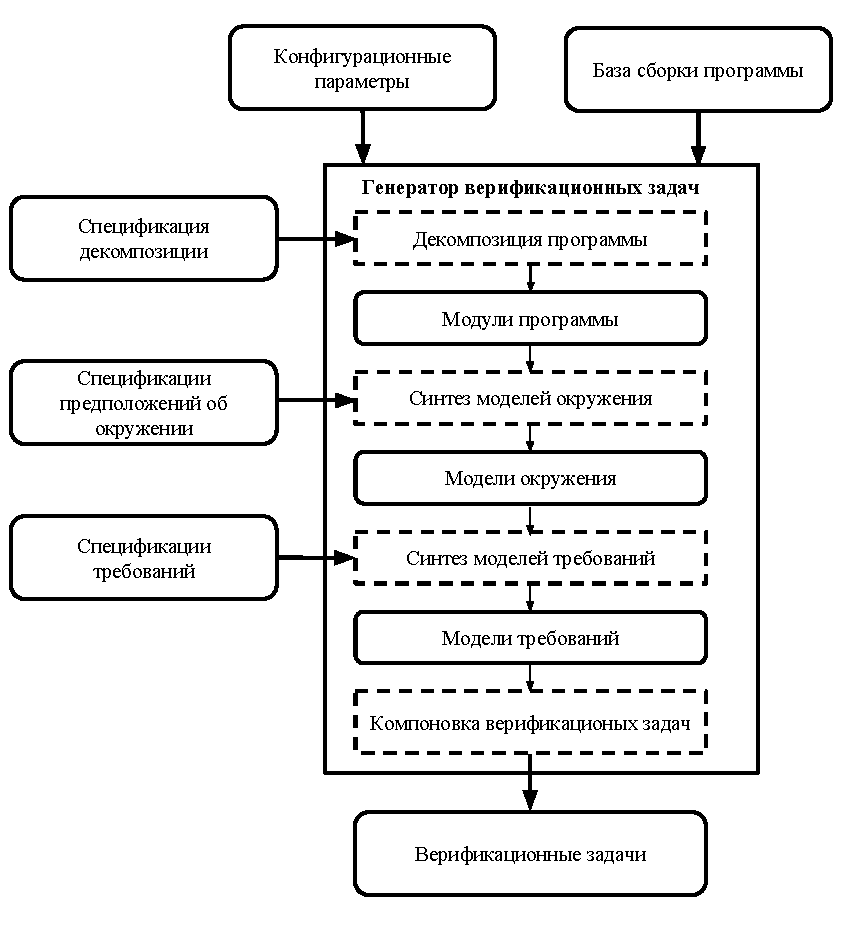
\includegraphics[scale=0.7]{vt_generator}
\caption{Структура генератора верификационных задач.}
\label{figure:vt_generator}
\end{figure}

Третий раздел рассматривает декомпозицию Си-программ.
При декомпозиции определяется та часть исходного кода программы, которую необходимо верифицировать, и в ней выделяются модули для генерации верификационных задач.

Перед выполнением верификации оценить результат декомпозиции затруднительно, так как на сегодняшний день нет надежных методов прогнозирования возможности решения верификационной задачи при заданных ограничениях на вычислительные ресурсы.
Поэтому декомпозицию предлагается выполнять автоматизированно с возможностью настройки процесса декомпозиции и коррекции состава модулей.

\textbf{Метод автоматизированной декомпозиции программ на модули} состоит в выполнении следующих шагов: определения файлов и функций в составе программы, выделения логических компонентов, выбора целевых модулей, коррекции состава модулей согласно спецификации декомпозиции и агрегации.
Входными данными являются конфигурационные параметры, где пользователь указывает часть программы, которую требуется верифицировать, база сборки и \textit{спецификация декомпозиции}, разработанная вручную пользователем для коррекции состава модулей, получаемых автоматически.

На шаге определения состава программы выполняется построение двух ориентированных графов на основе базы сборки: графа файлов и графа функций.
Вершины графов соответствуют файлам и функциям соответственно, а ребра отражают зависимости по вызову функций.

На следующем шаге выполняется деление множества вершин графа файлов на непересекающиеся подмножества, называемые модулями, согласно некоторой \textit{стратегии выделения модулей}.
Стратегия определяет специализированный алгоритм, предназначенный для выделения модулей в определенной программной системе.
Результатом деления является граф модулей, в котором вершины соответствуют модулям, а ребра отражают зависимости между ними по вызову функций.

Следующим шагом является выбор модулей, которые требуется верифицировать.
Такие модули называются целевыми и определяются при помощи конфигурационных параметров, в которых указаны пользователем целевые директории и файлы с исходным кодом, функции и модули.
Соответствующие им вершины графов модулей и файлов на данном шаге помечаются как целевые.

Если пользователь задал спецификацию декомпозиции, то выполняется коррекция состава модулей и соответствующего графа. 

На последнем шаге выполняется выбор наборов модулей в графе для каждого целевого модуля, минимизируя число точек входа совокупности модулей для сокращения трудоемкости моделирования для них окружения, согласно некоторой \textit{стратегии агрегации}.
Стратегия определяет специализированный алгоритм поиска наборов модулей в графе определенного вида.
Каждый набор модулей становится новым модулем, для которого будут сгенерированы верификационные задачи.

Предложенный метод позволяет адаптировать процесс декомпозиции к разным видам Си-программ при помощи конфигурирования и разработки новых стратегий и спецификаций декомпозиции.

В четвертом разделе изложен метод спецификации моделей окружения модулей Си-программ.

Для модулей с единственной точкой входа предлагается разрабатывать модели неопределенных функций на языке программирования Си.
Процесс моделирования окружения для библиотек и событийно-ориентированных программ требует построения композиции из моделей сценариев взаимодействия модуля и окружения.
Агрегация модулей программы позволяет снизить трудозатраты на моделирование, но при этом могут возникнуть новые требования к последовательностям событий разных сценариев взаимодействия, которые требуется учитывать при спецификации моделей окружения.

\textbf{Метод спецификации модели окружения} для некоторого модуля заключается в разработке \textit{промежуточной модели окружения}, которая определяется парой $M =~<P, E>$ и описывает модель окружения некоторой параллельной программы, использующей программный интерфейс управления потоками согласно стандарту POSIX.
$P$ состоит из множеств вспомогательных переменных, функций, макросов и типов, определенных на языке программирования Си.
$E$ содержит конечное множество моделей сценариев взаимодействия, которые делятся на два вида: \textit{модели функций окружения} и \textit{модели потоков окружения}.
Каждая модель функции окружения реализует модель сценария взаимодействия, события которого происходят во время выполнения некоторой функции, определенной в окружении.
Модель потока окружения реализует модель сценария взаимодействия, события которого выполняются в отдельном потоке.

Каждая модель сценария определяется системой переходов \break $\varepsilon =~<\mathcal{V}, \mathcal{A}, \alpha_0 ,\mathcal{R}>$.
Где $\mathcal{V}$ --- это множество переменных состояния, заданных на языке Си, $\mathcal{A}$ --- это множество \textit{действий}, $\alpha_0 \in \mathcal{A}$ называется начальным действием, а $\mathcal{R}:~ \mathcal{A}~\times~\mathcal{A}$ --- отношение переходов для задания ограничений на порядок следования действий.
Будем различать действия трех видов: \textit{прием сигнала}, \textit{отправка сигнала} и \textit{модель события}.

Каждая модель события описывается при помощи предусловия, постусловия и базового блока кода на языке программирования Си, состоящего из операций над переменными состояния и глобальными переменными модуля и модели окружения.
Базовые блоки содержат вызовы точек входа модулей и инициализацию параметров для них.
Действия передачи сигналов выполняются согласно модели синхронизации рандеву между парами моделей сценариев и служат для задания ограничений на порядок событий разных сценариев взаимодействия и на зависимости по данным между ними.

Промежуточная модель окружения компонуется вместе с исходным кодом модуля при помощи инструментации, поэтому семантика модели без модуля не определена.
Предложенные модели сценариев можно описывать на языке программирования Си.
Но для описания действий посылки и получения сигналов предлагается расширить язык Си вспомогательными операциями для удобства спецификации.
Поэтому промежуточные модели окружения перед верификацией модуля должны быть предварительно транслированы на язык программирования Си.
Необходимо показать, что трансляция промежуточной модели окружения не влияет на возможность обнаружения ошибок в модуле методом верификации моделей.
Для этого рассмотрен некоторый Си-подобный язык программирования $LZ$ и его расширение $ELZ$, полученное добавлением операций пересылки сигналов.
Языки сохраняют именно те особенности семантики программ на языке Си, на которые влияет добавление операций посылки и получения сигналов: порядок выполнения операций, синхронизацию потоков и передачу данных между ними, проверку логических выражений и целочисленную арифметику.
Семантика выполнения программ на данных языках задана при помощи символических систем переходов.

Затем были проанализированы свойства предложенной семантики выполнения программ на языках $LZ$ и $ELZ$, сформулированы и доказаны вспомогательные леммы и основная теорема:

\begin{lemma}
Истинность предиката пути, на котором могут выполняться подряд две независимые операции не зависит от порядка выполнения данных операций между собой.
\end{lemma}
\begin{lemma}
На эквивалентность блоков не влияют независимые операции выполняемые параллельно в других процедурах.
\end{lemma}
\begin{lemma}
Предикат пути через блоки кода с захваченной блокировкой принимает истинное значение только в том случае, если на этом пути операции между метками входа и выхода каждого блока под блокировкой может одновременно выполнять только один поток.
\end{lemma}
\begin{lemma}
На пути выполнения блока из операций $flag$ и $recv$ приема сигнала $d$ всегда происходит посылка данного сигнала из другого потока.
\end{lemma}
\begin{theorem}
Множества достижимых ошибочных состояний исходной программы на языке $ELZ$ и результата ее трансляции на язык $LZ$ изоморфны.  
\end{theorem}

Результат теоремы справедлив при проверке требований методом верификации моделей к программе на языке Си, сведенных к доказательству недостижимости ошибочного оператора, в предположениях, что программа использует только интерфейс управления потоками POSIX и инструмент при верификации строит модель с теми же свойствами, которыми обладают рассмотренные при доказательстве теоремы модели программ на языках $LZ$ и $ELZ$.

В пятом разделе описан \textbf{метод автоматизированного синтеза моделей окружения на языке программирования Си}, который заключается в построении моделей сценариев взаимодействия на основе спецификаций предположений об окружении, подготовке промежуточной модели окружения как композиции моделей сценариев взаимодействия и ее трансляции на язык Си.
Метод выполняется \textit{генератором моделей окружения}, структура которого изображена на рисунке~\ref{figure:em}.

\begin{figure}
\centering
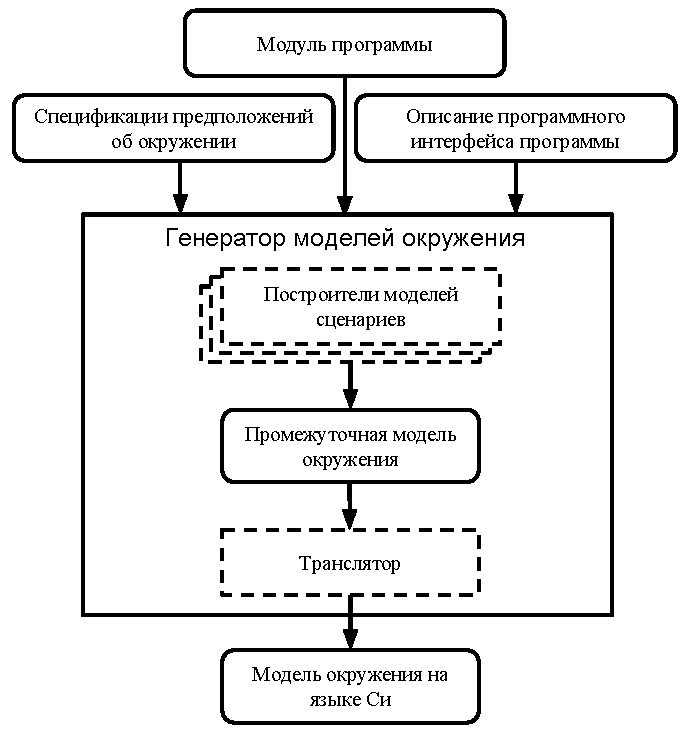
\includegraphics[scale=0.8]{generators}
\caption{Структура генератора моделей окружения.}
\label{figure:em}
\end{figure}

В зависимости от устройства верифицируемой программы используются несколько построителей моделей сценариев взаимодействия для промежуточной модели окружения.
Каждый построитель выполняет подготовку моделей сценариев на основе соответствующих спецификаций предположений об окружении и описания программного интерфейса из базы сборки программы.
Спецификации предположений об окружении содержат модели отдельных сценариев взаимодействия на разных языках предметной области, расширяющих формат задания промежуточной модели окружения для упрощения описания моделей сценариев определенного вида.

Затем выполняется трансляция промежуточной модели окружения на язык программирования Си.
Транслятор позволяет выполнять настройку процесса генерации модели окружения в зависимости от проверяемого требования и используемого инструмента верификации.

Шестой раздел описывает синтез моделей требований на основе спецификаций требований, разрабатываемых на аспектно-ориентированном расширении языка программирования Си, согласно методу, реализованному в системе верификации LDV~Tools.

В седьмом разделе рассматривается процесс компоновки верификационных задач в формате, предложенном сообществом SV"~COMP, из модулей программы и соответствующих синтезированных моделей окружения и требований. 
На практике на данном шаге выполняется препроцессирование, инструментация и построение среза исходного кода верификационной задачи (англ. slicing).

В \textbf{третьей главе} описана архитектура системы верификации моделей программ для генерации и решения верификационных задач с использованием распределенных вычислительных систем.

Структура системы верификации изображена на рисунке \ref{figure:system}. 
Сервер предназначен для организации взаимодействия пользователя и компонентов системы верификации, а также для хранения данных.
При помощи пользовательского интерфейса сервера пользователи формируют \textit{верификационные задания}, состоящие из базы сборки программы, спецификаций и конфигурационных параметров.
Генератор выполняет автоматическую подготовку верификационных задач для определенного верификационного задания согласно схеме, изложенной во второй главе. 
Инструменты верификации моделей программ решают верификационные задачи, подготовленные в рамках решения верификационных заданий.
Решатель верификационных задач и заданий предназначен для управления вычислительными ресурсами и запуска экземпляров остальных компонентов.

\begin{figure}
\centering
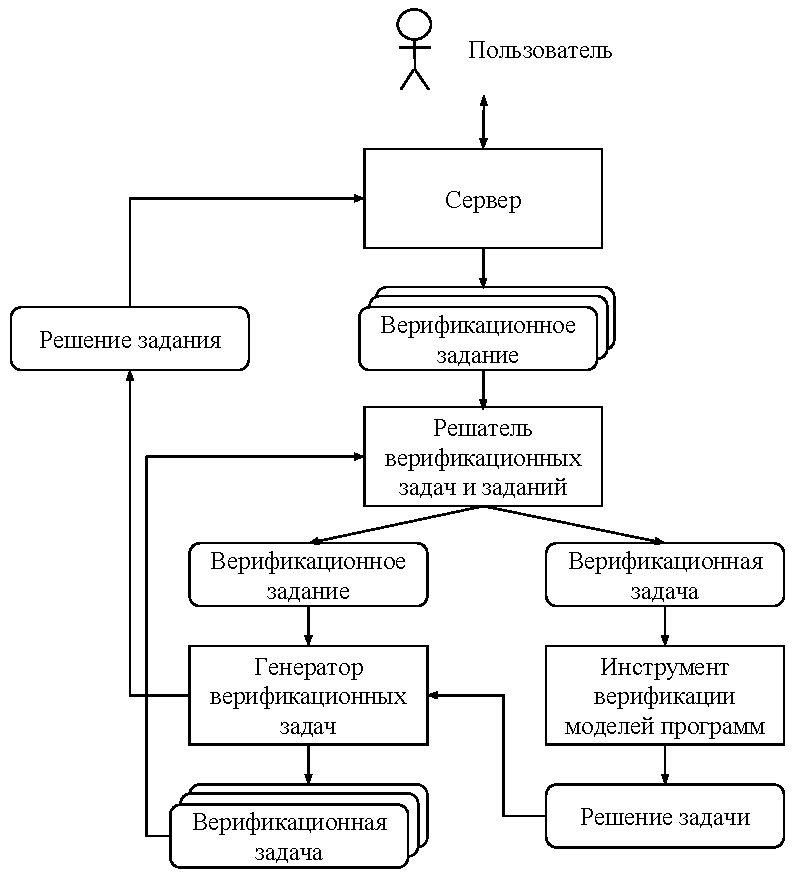
\includegraphics[scale=0.7]{system}
\caption{Структура системы верификации моделей программ.}
\label{figure:system}
\end{figure}

Каждое верификационное задание и задача имеют максимальное ограничение на вычислительные ресурсы: объем доступной оперативной памяти и памяти на диске, время выполнения и процессорное время.
Ограничения необходимо соблюдать для получения воспроизводимых результатов верификации.

При получении на вход верификационного задания или задачи решатель выполняет процедуру планирования и запуска экземпляров необходимых компонентов, выполняемую специальными модулями.
Модули предназначены обеспечить взаимодействие решателя с разными системами управления вычислительными кластерами и облачными сервисами.

В \textbf{четвертой главе} представлена реализация предложенных методов в системе верификации Klever.

Система верификации Klever является проектом с открытым исходным кодом и предназначена для проверки требований к программным системам на языке программирования Си с расширениями GNU при помощи инструментов верификации моделей программ.

Для программных систем BusyBox и ядра ОС Linux были разработаны специализированные стратегии выделения модулей.
Для агрегации модулей были реализованы алгоритмы, опирающиеся на граф вызова функций и отчеты о покрытии модулей при верификации.
В генераторе моделей окружения реализованы три построителя моделей сценариев, из которых два предназначены для верификации драйверов и подсистем ядра ОС Linux, а третий может быть использован для различных программ.
В данном компоненте реализован конфигурируемый транслятор, поддерживающий построение последовательной или параллельной модели окружения.
Синтез моделей требований выполнен с возможностью использования спецификаций требований, разработанных для системы верификации LDV~Tools.
Инструментация исходного кода в компоновщике реализована при помощи инструмента CIF (C Instrumentation Framework), основанного на компиляторе GCC версии 7.1.
Построение среза исходного кода верификационной задачи выполняется при помощи CIL из набора инструментов по дедуктивной верификации Си-программ AstraVer Toolset.

Решатель реализован с поддержкой решения верификационных задач на одном вычислительном узле или в вычислительном кластере, управляемом при помощи  VerifierCloud.

Система позволяет применять инструменты верификации моделей Си-программ, поддерживающие формат верификационных задач сообщества \break SV"~COMP.
На практике используются различные версии инструментов верификации CPAchecker и Ultimate Automizer.

В \textbf{пятой главе} представлены результаты практического применения предложенных методов, реализованных в системе верификации Klever, а также сделаны выводы о границах их практической применимости.

Предложенные в данной работе методы нацелены преимущественно на сокращение трудоемкости и скорости верификации, а уровень точности верификации не должен понизиться.
Во втором разделе анализируются результаты экспериментов по верификации драйверов и подсистем ОС Linux и приводятся оценки улучшения характеристик, достигнутых при помощи разработанных методов.

На первом этапе выполнения экспериментов, чтобы оценить трудоемкость верификации для получения результатов с высоким уровнем точности, был выбран набор из 49 Serial драйверов ОС Linux версии 3.14.79, размер исходного кода которых составляет 30 тыс. строк кода.
Затем рассматривается переход к верификации остальных драйверов ОС Linux, размер которых составляет более 3 млн. строк кода, и оцениваются дополнительные трудозатраты.
На заключительном этапе выполняется верификация подсистем без разработки новых спецификаций, чтобы подтвердить возможность повторного использования имеющихся артефактов.
Оценка трудоемкости всех трех этапов представлена в таблице~\ref{table:difficulty}\footnote{Разработка спецификаций требований выполнялась за рамками данной работы, а оценка трудоемкости приведена для полноты описания процесса подготовки к верификации.}.
 
Для измерения времени верификации проверялись наборы из 49 Serial и 3864 других драйверов на соответствие 30 требованиям.
Результаты, представленные в таблице~\ref{table:speed}, были получены с использованием 2-х физ. ядер, 4-х физ. ядер и вычислительного кластера из 30 узлов с 4-я физ. ядрами в каждом.

Уровень покрытия по функциям при верификации драйверов составил 100\% для набора Serial и 45\% для остальных драйверов.
Чтобы достичь более высокого уровня необходимо затратить существенно больше усилий на разработку спецификаций предположений об окружении.
В то же время при помощи системы верификации Klever уже было выявлено более ста ошибок в различных драйверах.

В таблице~\ref{table:serialldv} представлены результаты сравнительного анализа вердиктов, полученных при верификации Serial драйверов при помощи систем верификации Klever и LDV~Tools.
Проверка требований корректности работы с памятью и отсутствия гонок по данным возможна только в системе верификации Klever благодаря конфигурируемости генератора моделей окружения, а остальные 30 проверяемых требований совпадают.
Результаты демонстрируют, что система верификации Klever позволяет получить меньше ложных предупреждений об ошибках в связи с повышением уровня точности моделей окружения, а также позволяет выявить новые ошибки.

Чтобы выяснить, как на результаты верификации влияет проверка разных версий ядра ОС Linux с одним и тем же набором спецификаций, были рассмотрены подсистемы GPIO, TTY и CHAR версий ядра ОС Linux, начиная с 3.9 и заканчивая 3.19.
На рисунке~\ref{figure:verdicts} представлено среднее число полученных вердиктов в зависимости от версии ядра для каждой подсистемы.
Были проанализированы вручную 488 изменений в упомянутых подсистемах, чтобы выявить исправления ошибок, которые являются нарушениями формализованных в рамках системы верификации Klever требований.
Среди 8 таких исправлений ошибок, 4 могут быть успешно выявлены системой верификации, две ошибки не относятся к рассматриваемым конфигурации и архитектуре, а еще две были пропущены из-за ограничений инструмента верификации.

В третьем разделе исследуется возможность применения системы верификации Klever к пользовательским программам.
Для этого выполнены эксперименты по верификации апплетов проекта BusyBox, которые являются пользовательскими преобразующими программами с единственной точкой входа.
Трудоемкость подготовки к верификации представлена в таблице~\ref{busybox:difficulty}, а статистика по полученным вердиктами в таблице~\ref{table:busy}.
Уровень покрытия по функциям составил 94\%.


\begin{table}
\centering
\begin{tabular}{ | l | c | c | c |}
\hline
Этап разработки& Serial Драйверы & Все драйверы & Подсистемы\\
\hline
\shortstack[l]{Стратегий \\ декомпозиции} & 
\shortstack[c]{0,25 чел. мес. \\ 100LOC Python} & 
\shortstack[c]{0 чел. мес. \\ 100LOC Python} &
\shortstack[c]{0,25 чел. мес. \\ 120LOC Python} \\
\hline
\shortstack[l]{Построителей \\ моделей сценариев} & 
\shortstack[c]{3 чел. мес. \\ 3KLOC Python} &
\shortstack[c]{0 чел. мес. \\ 3KLOC Python} &
\shortstack[c]{0,5 чел. мес. \\ 3,5KLOC Python} \\
\hline
\shortstack[l]{Спецификаций \\ предположений \\об окружении} & 
\shortstack[c]{4,5 чел. мес. \\ 7KLOC DSL} &
\shortstack[c]{5,5 чел. мес. \\ 17KLOC DSL} &
\shortstack[c]{0 чел. мес. \\ 17KLOC DSL} \\
\hline
\shortstack[l]{Спецификаций \\ требований} &
\shortstack[c]{6 чел. мес. \\ 550LOC DSL} &
\shortstack[c]{9 чел. мес. \\ 1500LOC DSL} & 
\shortstack[c]{0,25 чел. мес. \\ 1500LOC DSL} \\
\hline
\textbf{Итого} & 13,75 чел. мес. & 14,5 чел. мес. & 1 чел. мес. \\
\hline
\end{tabular}
\caption{Трудоемкость верификации драйверов и подсистем ОС Linux.}
\label{table:difficulty}
\end{table}

\begin{table}
\centering
\begin{tabular}{| l | c | c | c |}
\hline
Верификационное задание & 2 физ. ядра & 4 физ. ядра & 30 * 4 физ. ядра \\
\hline 
Serial драйверы (30KLOC) & 5ч & 2,7ч & 0,5ч \\
\hline 
Все драйверы (3MLOC) & 600ч & 195ч & 11ч \\
\hline
\end{tabular}
\caption{Время верификации драйверов ОС Linux версии 3.14.79.}
\label{table:speed}
\end{table}

\begin{table}
\centering
\begin{tabular}{| l | c | c | c | c |}
\hline
\shortstack[l]{Верификационное \\ задание} &
\shortstack[l]{Ложное \\ предупреждение} &
Ошибка & Нет вердикта\\
\hline
\shortstack[l]{Klever, 32 требования} & 16 & 6 & 46\\ 
\hline
\shortstack[l]{Klever, 30 требований} & 5 & 1 & 16\\ 
\hline
\shortstack[l]{LDV Tools, 30 набор требований} & 31 & 0 & 9\\
\hline
\end{tabular}
\caption{Вердикты при верификации Serial драйверов ОС Linux версии 3.14.79.}
\label{table:serialldv}
\end{table}

\begin{figure}
\centering
\begin{tikzpicture}
\begin{axis}[
  width=13cm,
  height=7cm,
  grid=major,
  xlabel=Версия ядра Linux,
  ylabel=Среднее число вердиктов,
  xtick=data,
  xticklabels={3.9,3.10,3.11,3.12,3.13,3.14,3.15,3.16,3.17,3.18,3.19},
  legend style={
    at={(0.95,0.5)},
    anchor=west
  }
]
\addplot[blue,mark=*]         coordinates {(0,9.0) (1,9.0) (2,9.0) (3,9.0) (4,9.0) (5,9.0) (6,9.0) (7,9.0) (8,9.0) (9,9.0) (10,9.0)};
\addlegendentry{CHAR True}
\addplot[red,mark=*]          coordinates {(0,9.0) (1,8.1) (2,8.8) (3,8.6) (4,8.6) (5,8.7) (6,8.8) (7,9.8) (8,8.8) (9,8.8) (10,10.2)};
\addlegendentry{GPIO True}
\addplot[brown,mark=*]        coordinates {(0,7.4) (1,7.4) (2,7.4) (3,7.4) (4,7.4) (5,7.4) (6,7.4) (7,7.4) (8,7.4) (9,7.5) (10,7.5)};
\addlegendentry{TTY True}
\addplot[blue,mark=square*]   coordinates {(0,0.0) (1,0.0) (2,0.0) (3,0.0) (4,0.0) (5,0.0) (6,0.0) (7,0.0) (8,0.0) (9,0.0) (10,0.0)};
\addlegendentry{CHAR False}
\addplot[red,mark=square*]    coordinates {(0,0.5) (1,0.5) (2,0.5) (3,0.5) (4,0.5) (5,0.6) (6,0.9) (7,0.8) (8,1.8) (9,1.7) (10,0.5)};
\addlegendentry{GPIO False}
\addplot[brown,mark=square*]  coordinates {(0,0.6) (1,0.3) (2,0.3) (3,0.7) (4,0.8) (5,0.7) (6,0.7) (7,0.7) (8,0.7) (9,0.6) (10,0.3)};
\addlegendentry{TTY False}
\addplot[blue,mark=diamond*]  coordinates {(0,3.0) (1,3.0) (2,3.0) (3,3.0) (4,3.0) (5,3.0) (6,3.0) (7,3.0) (8,3.0) (9,3.0) (10,3.0)};
\addlegendentry{CHAR Unknown}
\addplot[red,mark=diamond*]   coordinates {(0,2.5) (1,3.4) (2,2.8) (3,2.9) (4,2.9) (5,2.7) (6,2.3) (7,1.4) (8,1.5) (9,1.5) (10,1.2)};
\addlegendentry{GPIO Unknown}
\addplot[brown,mark=diamond*] coordinates {(0,4.0) (1,4.3) (2,4.3) (3,3.9) (4,3.8) (5,3.9) (6,3.9) (7,3.9) (8,3.9) (9,3.9) (10,4.2)};
\addlegendentry{TTY Unknown}
\end{axis}
\end{tikzpicture}
\caption{Среднее число вердиктов при верификации целевых подсистем в зависимости от версии ОС Linux.}
\label{figure:verdicts}
\end{figure}

\begin{table}
\centering
\begin{tabular}{ | c | c | c | c | c |}
\hline 
\shortstack[l]{Разработка \\ стратегий \\ декомпозиции} &
\shortstack[l]{Разработка \\ построителей \\ моделей сценариев} &
\shortstack[l]{Спецификация \\ предположений \\об окружении} & 
\shortstack[l]{Спецификация \\ требований} \\
\hline
\shortstack[c]{0,25 чел. мес. \\ 100LOC Python} & 
\shortstack[c]{0 чел. мес.} &
\shortstack[c]{0,25 чел. мес. \\ 200LOC DSL} &
\shortstack[c]{0,5 чел. мес. \\ 300LOC DSL} \\
\hline
\end{tabular}
\caption{Трудоемкость верификации апплетов проекта BusyBox.}
\label{busybox:difficulty}
\end{table}

\begin{table}
\centering
\begin{tabular}{| l | c | c | c | c |}
\hline
\shortstack[l]{Верификационное \\ задание} &
\shortstack[l]{Ложное \\ предупреждение} & Ошибка & Нет ошибок & Нет вердикта\\
\hline
BusyBox (200KLOC) & 6 & 1 & 159 & 133 \\
\hline
\end{tabular}
\caption{Вердикты, полученные при верификации апплетов проекта BusyBox.}
\label{table:busy}
\end{table}

В последнем разделе делаются выводы о пределах применимости разработанных методов и системы верификации, а также делается заключение о целесообразности их использования при верификации программных систем, имеющих событийно-ориентированное архитектуру, например, операционных систем, веб-серверов и встраиваемого программного обеспечения.

% Заключение
В \textbf{Заключении} представлены основные результаты работы.

\nsection{Основные результаты работы}

Основные научные результаты, полученные в диссертационной работе и выносимые на защиту, состоят в следующем:
\begin{itemize}
    \item Разработан метод автоматизированной декомпозиции Си-программ на модули.
    \item Разработан метод спецификации моделей окружения модулей на основе композиции систем переходов.
    \item Разработан метод автоматизированного синтеза моделей окружения модулей, позволяющий адаптировать процесс синтеза для проверки разных видов требований и программ.
\end{itemize}

На основе предлагаемых методов была реализована система верификации Klever, предназначенная для проверки требований к программным системам на языке программирования Си с расширениями GNU методом верификации моделей программ.
Продемонстрировано, что разработанная архитектура системы верификации позволяет проводить верификацию на различных многоядерных и распределенных вычислительных системах.

% ----------------------------------------------------------------
\printbibliography[heading=authorcited,keyword={mypaper}, resetnumbers=true]

% ----------------------------------------------------------------
% Пример выходных данных
%\clearpage
%\thispagestyle{empty}
%\normalfont\selectfont
%\vspace*{2cm}
%\begin{center}
%\textit{Научное издание}\\
%\vskip 2cm
%\makeatletter
%\@author
%\vskip 1.5cm
%\@title{} на тему:\\
%\@topic\\
%\makeatother
%\end{center}
%\vfill
%Подписано в печать~25.01.2011.
%Формат~$60 \times 90$~1/16.
%Тираж~100~экз.
%Заказ~256.\\[2ex]
%\noindent
%Санкт-Петербургская издательская фирма <<Наука>> РАН.
%199034, Санкт-Петербург, Менделеевская линия, 1,
%\href{http://www.naukaspb.spb.ru}{http://www.naukaspb.spb.ru}
\end{document}
